\scanpage{79}
interpréter la structure polygonale sur
l'ens des $a_\alpha$, en termes des $a'_\alpha$
correspondants. Notons déjà qu'il y
a correspondance entre les \deleted{\unsure{structures}} \inserted{orientations}
de $F$, et celles de $D$, et que le
transport continu de l'orientation de
$F$ vers une face adjacente $F'$
(le long de $a_\alpha$ disons) correspond au
transport continu (ou ``parallèle'') de
l'orientation de $D$ au cours du balayage
correspondant. \deleted{\unsure{(D}} Ce dernier point
rend plausible le choix ``naïf'' du
transport d'orientation, qui dans le contexte
des \unsure{modèles} de \unsure{p.v.} obtenus via balayage,
semble en effet meilleur, du pt de
vue ``circuits''. Le fait qu'on n'obtienne
pas d'application naturelle $\unsure{\mathcal X}\to X$ se
rapproche du fait qu'on n'a pas d'application
naturelle $X^\vee\to X$.

\figure{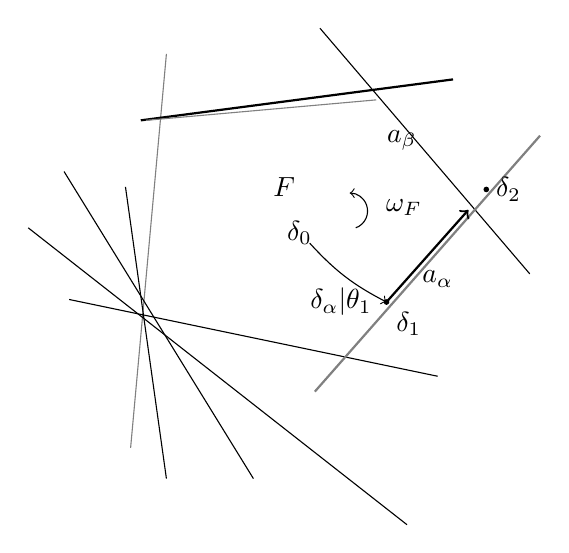
\begin{tikzpicture}[x=.65cm,y=.65cm]
\draw[gray] (1.8,0.8)--(2.5,8.5);
\draw (1.7,5.9)--(2.5,.2);
\draw (.5,6.2)--(4.2,.2);
\draw (-.2,5.1)--(7.2,-.7);
\draw (.6,3.7)--(7.8,2.2);
\draw[thick] (2,7.2)--(8.1,8);
\draw[gray] (2.1,7.2)--(6.6,7.6);
\draw (5.5,9)--(9.6,4.2);
\draw[gray,thick] (5.4,1.9)--(9.8,6.9);
\draw[->,thick] (6.8,3.65)--(8.4,5.45);
\fill (6.8,3.65) circle (.055) node[below right] {$\delta_1$};
\fill (8.75,5.85) circle (.055) node[right] {$\delta_2$};
\node at (7.1,6.8) {$a_\beta$};
\node at (7.8,4.1) {$a_\alpha$};
\node at (4.8,5.9) {$F$};
\node at (5.1,5) {$\delta_0$};
\draw[->] (5.3,4.8) to[bend right=10] (6.8,3.65);
\node[left] at (6.7,3.65) {$\unsure{\delta_\alpha|\theta_1}$};
\draw[->] (6.2,5.1) arc[start angle=-70,end angle=90,radius=.35];
\node[right] at (6.6,5.5) {$\omega_F$};
\end{tikzpicture}}

\figure{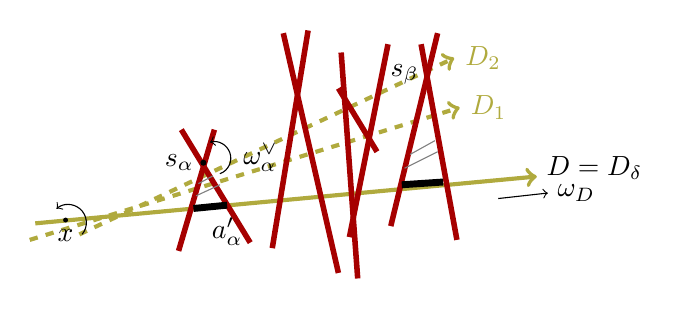
\begin{tikzpicture}[x=.7cm,y=.7cm]
\draw[yellow!65!black,line width=1.5pt,->] (0,.8)--(9.1,1.65);
\node[right] at (9.1,1.8) {$D=D_{\unsure{\delta}}$};
\draw[->] (8.4,1.25)--(9.3,1.35) node[right] {$\omega_D$};
\draw[yellow!65!black,line width=1.5pt,dashed,->] (-.1,.5)--(7.7,2.9) node[right] {$D_1$};
\draw[yellow!65!black,line width=1.5pt,dashed,->] (.8,.6)--(7.6,3.8) node[right] {$D_2$};
\draw[red!65!black,line width=2pt] (2.6,.3)--(3.25,2.5);
\draw[red!65!black,line width=2pt] (2.65,2.5)--(3.9,.45);
\draw[red!65!black,line width=2pt] (4.3,.35)--(4.95,4.3);
\draw[red!65!black,line width=2pt] (4.5,4.25)--(5.5,-.1);
\draw[red!65!black,line width=2pt] (5.55,3.9)--(5.85,-.2);
\draw[red!65!black,line width=2pt] (5.7,.55)--(6.4,4.05);
\draw[red!65!black,line width=2pt] (5.5,3.25)--(6.2,2.1);
\draw[red!65!black,line width=2pt] (6.45,.75)--(7.3,4.25);
\draw[red!65!black,line width=2pt] (7,4.05)--(7.65,.5);
\draw[line width=2.5pt] (2.87,1.07)--(3.48,1.13) node[below] {$a'_\alpha$};
\draw[line width=2.5pt] (6.65,1.5)--(7.4,1.55);
\draw[gray] (2.92,1.3)--(3.35,1.5);
\draw[gray] (2.96,1.52)--(3.22,1.66);
\draw[gray] (6.7,1.8)--(7.3,2.1);
\draw[gray] (6.8,2.05)--(7.25,2.3);
\fill (3.05,1.9) circle (.055) node[left] {$s_\alpha$};
\node[left] at (7.13,3.5) {$s_\beta$};
\fill (.55,.86) circle (.045) node[below] {$x$};
\draw[->] (.85,.6) arc[start angle=-40,end angle=130,radius=.33];
\draw[->] (3.35,1.7) arc[start angle=-70,end angle=105,radius=.3];
\node[right] at (3.6,2) {$\omega_\alpha^\vee$};
\end{tikzpicture}}

Partons avec une orientation $\omega_F$ de
$F$ ($\mapsto\omega_D$ de $D$) et une
arête $a_\alpha$ ($\mapsto s_\alpha$ sommet de $\Sigma$)
allant de $\delta_0\in F$ ($\mapsto D=D_{\delta_0}$) en
ligne droite vers un pt $\delta_1$ voisin de
$a_\alpha$ --- i.e. \unsure{faisons} \unsure{choisissons}
un pt $x$ sur $D$ et une orientation
de rotation en $x$, et faisons pivoter
\margin{78}
